% Paper de P v2 (Springer LNCS). Compilar desde esta carpeta:  latexmk -pdf paper_v2.tex
\documentclass[runningheads]{llncs}
\usepackage[T1]{fontenc}
\usepackage[utf8]{inputenc}
\usepackage[spanish,es-tabla,es-nodecimaldot]{babel}
\usepackage{amsmath,amssymb}
\usepackage{graphicx}
\usepackage{booktabs}
\usepackage{xcolor}
\usepackage{tikz}
\usetikzlibrary{arrows.meta,positioning}
\usepackage[hidelinks]{hyperref}
\definecolor{azulm}{HTML}{2E6DB4}\definecolor{naranjam}{HTML}{D9731A}
\definecolor{verdem}{HTML}{2F9467}\definecolor{grism}{HTML}{5A6772}
\graphicspath{{../figuras/}{../../final/figuras/}}
% Generado por analisis.py: NO editar a mano.
\newcommand{\nDatasets}{12}
\newcommand{\nParticiones}{5}
\newcommand{\nCasos}{60}
\newcommand{\relRL}{0{,}96}
\newcommand{\cambioRL}{$-$4{,}4\,\%}
\newcommand{\casosRL}{36/60}
\newcommand{\dsRL}{7/12}
\newcommand{\pRL}{$1{,}000$}
\newcommand{\cambioVsEstRL}{$-$2{,}6\,\%}
\newcommand{\dsVsEstRL}{6/12}
\newcommand{\pVsEstRL}{$1{,}000$}
\newcommand{\peorDsRL}{$+$20{,}9\,\%}
\newcommand{\relKNN}{0{,}76}
\newcommand{\cambioKNN}{$-$24{,}3\,\%}
\newcommand{\casosKNN}{56/60}
\newcommand{\dsKNN}{12/12}
\newcommand{\pKNN}{$0{,}004$}
\newcommand{\cambioVsEstKNN}{$-$13{,}6\,\%}
\newcommand{\dsVsEstKNN}{10/12}
\newcommand{\pVsEstKNN}{$0{,}048$}
\newcommand{\peorDsKNN}{$-$0{,}4\,\%}
\newcommand{\relArbol}{1{,}00}
\newcommand{\cambioArbol}{$+$0{,}1\,\%}
\newcommand{\casosArbol}{34/60}
\newcommand{\dsArbol}{7/12}
\newcommand{\pArbol}{$1{,}000$}
\newcommand{\cambioVsEstArbol}{$+$0{,}1\,\%}
\newcommand{\dsVsEstArbol}{7/12}
\newcommand{\pVsEstArbol}{$1{,}000$}
\newcommand{\peorDsArbol}{$+$5{,}0\,\%}
\newcommand{\relRF}{1{,}00}
\newcommand{\cambioRF}{$+$0{,}5\,\%}
\newcommand{\casosRF}{27/60}
\newcommand{\dsRF}{5/12}
\newcommand{\pRF}{$1{,}000$}
\newcommand{\cambioVsEstRF}{$+$0{,}5\,\%}
\newcommand{\dsVsEstRF}{5/12}
\newcommand{\pVsEstRF}{$1{,}000$}
\newcommand{\peorDsRF}{$+$4{,}1\,\%}
\newcommand{\cambioSintRL}{$-$1{,}3\,\%}
\newcommand{\pSintRL}{$0{,}705$}
\newcommand{\dsSintRL}{7/12}
\newcommand{\relSintRL}{0{,}99}
\newcommand{\cambioSintKNN}{$-$0{,}3\,\%}
\newcommand{\pSintKNN}{$0{,}705$}
\newcommand{\dsSintKNN}{7/12}
\newcommand{\relSintKNN}{1{,}00}
\newcommand{\cambioSintArbol}{$+$0{,}3\,\%}
\newcommand{\pSintArbol}{$1{,}000$}
\newcommand{\dsSintArbol}{7/12}
\newcommand{\relSintArbol}{1{,}00}
\newcommand{\cambioSintRF}{$-$0{,}1\,\%}
\newcommand{\pSintRF}{$1{,}000$}
\newcommand{\dsSintRF}{7/12}
\newcommand{\relSintRF}{1{,}00}
\newcommand{\cambioRedRL}{$+$1{,}8\,\%}
\newcommand{\pRedRL}{$0{,}380$}
\newcommand{\dsRedRL}{5/12}
\newcommand{\relRedRL}{1{,}02}
\newcommand{\cambioRedKNN}{$+$1{,}0\,\%}
\newcommand{\pRedKNN}{$0{,}330$}
\newcommand{\dsRedKNN}{4/12}
\newcommand{\relRedKNN}{1{,}01}
\newcommand{\cambioRedArbol}{$+$1{,}4\,\%}
\newcommand{\pRedArbol}{$0{,}330$}
\newcommand{\dsRedArbol}{3/12}
\newcommand{\relRedArbol}{1{,}01}
\newcommand{\cambioRedRF}{$+$2{,}8\,\%}
\newcommand{\pRedRF}{$0{,}049$}
\newcommand{\dsRedRF}{1/12}
\newcommand{\relRedRF}{1{,}03}
\newcommand{\dimMedia}{83\,\%}
\newcommand{\fracEliminados}{22\,\%}
\newcommand{\dimMin}{38\,\%}
\newcommand{\dimMax}{92\,\%}
\newcommand{\mMedia}{0{,}4}
\newcommand{\fracConSintesis}{25\,\%}
\newcommand{\tauMediana}{0{,}18}
\newcommand{\casosNmenosUno}{38/60}
\newcommand{\wLat}{2{,}91}
\newcommand{\wLon}{2{,}85}
\newcommand{\wPop}{0{,}03}
\newcommand{\wInc}{0{,}41}
\newcommand{\fracApagados}{10\,\%}
\newcommand{\nCompCasos}{60}
\newcommand{\compMLKRRL}{$-$1{,}8\,\%}
\newcommand{\compMLKRKNN}{$-$22{,}5\,\%}
\newcommand{\compMLKRArbol}{$+$2{,}0\,\%}
\newcommand{\compMLKRRF}{$+$2{,}6\,\%}
\newcommand{\rangoMLKR}{5{,}7}
\newcommand{\compPGRL}{$-$15{,}7\,\%}
\newcommand{\compPGKNN}{$-$18{,}0\,\%}
\newcommand{\compPGArbol}{$+$0{,}7\,\%}
\newcommand{\compPGRF}{$+$0{,}8\,\%}
\newcommand{\rangoPG}{4{,}6}
\newcommand{\compYJMVRL}{$+$2{,}4\,\%}
\newcommand{\compYJMVKNN}{$-$14{,}5\,\%}
\newcommand{\compYJMVArbol}{$+$1{,}5\,\%}
\newcommand{\compYJMVRF}{$+$1{,}7\,\%}
\newcommand{\rangoYJMV}{5{,}0}
\newcommand{\compCuantRL}{$+$8{,}1\,\%}
\newcommand{\compCuantKNN}{$-$11{,}8\,\%}
\newcommand{\compCuantArbol}{$+$0{,}1\,\%}
\newcommand{\compCuantRF}{$+$0{,}0\,\%}
\newcommand{\rangoCuant}{6{,}4}
\newcommand{\compEstPCARL}{$-$1{,}8\,\%}
\newcommand{\compEstPCAKNN}{$-$12{,}4\,\%}
\newcommand{\compEstPCAArbol}{$-$0{,}6\,\%}
\newcommand{\compEstPCARF}{$-$1{,}9\,\%}
\newcommand{\rangoEstPCA}{4{,}6}
\newcommand{\compPCAnoventaRL}{$+$0{,}6\,\%}
\newcommand{\compPCAnoventaKNN}{$-$10{,}4\,\%}
\newcommand{\compPCAnoventaArbol}{$+$19{,}3\,\%}
\newcommand{\compPCAnoventaRF}{$+$17{,}9\,\%}
\newcommand{\rangoPCAnoventa}{8{,}1}
\newcommand{\compPCAcvRL}{$-$1{,}0\,\%}
\newcommand{\compPCAcvKNN}{$-$12{,}0\,\%}
\newcommand{\compPCAcvArbol}{$+$18{,}7\,\%}
\newcommand{\compPCAcvRF}{$+$15{,}1\,\%}
\newcommand{\rangoPCAcv}{7{,}4}
\newcommand{\compPsrRL}{$-$6{,}1\,\%}
\newcommand{\compPsrKNN}{$-$25{,}0\,\%}
\newcommand{\compPsrArbol}{$-$1{,}1\,\%}
\newcommand{\compPsrRF}{$-$2{,}3\,\%}
\newcommand{\rangoPsr}{3{,}2}
\newcommand{\compPRL}{$-$4{,}4\,\%}
\newcommand{\compPKNN}{$-$24{,}3\,\%}
\newcommand{\compPArbol}{$+$0{,}1\,\%}
\newcommand{\compPRF}{$+$0{,}5\,\%}
\newcommand{\rangoP}{4{,}7}
\newcommand{\mejorAlt}{estándar + PCA}
\newcommand{\rangoMejorAlt}{4{,}6}
\newcommand{\nReps}{10}
\newcommand{\vMedia}{0{,}80}
\newcommand{\vFracUno}{22\,\%}
\newcommand{\nSintMedia}{3{,}9}
\newcommand{\ctrlIniAleat}{$+$0{,}6\,\%}
\newcommand{\pCtrlIniAleat}{$1{,}000$}
\newcommand{\ctrlIniAleatRL}{$+$1{,}7\,\%}
\newcommand{\ctrlSigmaBajo}{$+$0{,}5\,\%}
\newcommand{\pCtrlSigmaBajo}{$1{,}000$}
\newcommand{\ctrlSigmaBajoRL}{$-$0{,}1\,\%}
\newcommand{\ctrlSigmaAlto}{$+$0{,}9\,\%}
\newcommand{\pCtrlSigmaAlto}{$1{,}000$}
\newcommand{\ctrlSigmaAltoRL}{$-$0{,}4\,\%}
\newcommand{\ctrlPobDoble}{$+$0{,}2\,\%}
\newcommand{\pCtrlPobDoble}{$1{,}000$}
\newcommand{\ctrlPobDobleRL}{$-$0{,}2\,\%}
\newcommand{\nAblCasos}{24}
\newcommand{\ctrlPesos}{$+$2{,}2\,\%}
\newcommand{\ctrlPesosRL}{$+$6{,}5\,\%}
\newcommand{\pCtrlPesos}{$0{,}424$}
\newcommand{\ctrlExp}{$+$10{,}0\,\%}
\newcommand{\ctrlExpRL}{$+$2{,}2\,\%}
\newcommand{\pCtrlExp}{$0{,}012$}
\newcommand{\ctrlAleat}{$+$6{,}2\,\%}
\newcommand{\ctrlAleatRL}{$+$3{,}0\,\%}
\newcommand{\pCtrlAleat}{$0{,}012$}
\newcommand{\ctrlMI}{$+$14{,}9\,\%}
\newcommand{\ctrlMIRL}{$+$6{,}8\,\%}
\newcommand{\pCtrlMI}{$0{,}012$}
\newcommand{\ctrlYJMI}{$+$11{,}0\,\%}
\newcommand{\ctrlYJMIRL}{$+$10{,}3\,\%}
\newcommand{\pCtrlYJMI}{$0{,}014$}
\newcommand{\nCtrlCasos}{24}
\newcommand{\rangoCeroR}{$+$2{,}2\,\%}
\newcommand{\pRangoCero}{$1{,}000$}
\newcommand{\dsPeorRangoCero}{7}
\newcommand{\rangoUnoR}{$+$0{,}3\,\%}
\newcommand{\pRangoUno}{$1{,}000$}
\newcommand{\dsPeorRangoUno}{6}
\newcommand{\rangoCuatroR}{$+$0{,}5\,\%}
\newcommand{\pRangoCuatro}{$1{,}000$}
\newcommand{\dsPeorRangoCuatro}{7}
\newcommand{\rangoOchoR}{$+$1{,}7\,\%}
\newcommand{\pRangoOcho}{$0{,}256$}
\newcommand{\dsPeorRangoOcho}{9}
\newcommand{\bordeUno}{11\,\%}
\newcommand{\bordeDos}{7\,\%}
\newcommand{\bordeCuatro}{8\,\%}
\newcommand{\bordeOcho}{5\,\%}
\newcommand{\nRango}{24}
\newcommand{\mleFueraDos}{24\,\%}
\newcommand{\nAlgCasos}{24}
\newcommand{\rangoCMA}{1{,}9}
\newcommand{\algMejor}{CMA-ES}
\newcommand{\algKNNcma}{$-$25{,}7\,\%}
\newcommand{\algKNNaleat}{$-$21{,}0\,\%}
\newcommand{\algKNNmin}{$-$24{,}8\,\%}
\newcommand{\algKNNmax}{$-$23{,}3\,\%}
\newcommand{\segMediana}{191}
\newcommand{\segMax}{243}
\newcommand{\msPorEval}{191}
\newcommand{\segMLKR}{16{,}8}
\newcommand{\segPG}{6{,}1}
\newcommand{\segYJMV}{0{,}6}
\newcommand{\popMin}{11}
\newcommand{\popMax}{13}
\newcommand{\muMin}{5}
\newcommand{\muMax}{6}
\newcommand{\muEffMin}{3{,}4}
\newcommand{\muEffMax}{4{,}0}
\newcommand{\genMin}{77}
\newcommand{\genMax}{91}
\newcommand{\nParadaPresupuesto}{12}
\newcommand{\nParadaTotal}{12}
\newcommand{\evalMejorMediana}{971}
\newcommand{\evalMejorMin}{658}
\newcommand{\mejoraFitnessMediana}{$-$12{,}1\,\%}
\newcommand{\sigmaFinMin}{0{,}007}
\newcommand{\sigmaFinMax}{0{,}06}
\newcommand{\cribSelRL}{$-$2{,}5\,\%}
\newcommand{\cribSelKNN}{$-$23{,}9\,\%}
\newcommand{\cribSelArbol}{$+$0{,}1\,\%}
\newcommand{\cribSelRF}{$+$0{,}8\,\%}
\newcommand{\cribDimSel}{72\,\%}
\newcommand{\cribFijoRL}{$-$5{,}4\,\%}
\newcommand{\cribFijoKNN}{$-$25{,}0\,\%}
\newcommand{\cribFijoArbol}{$-$0{,}5\,\%}
\newcommand{\cribFijoRF}{$+$0{,}0\,\%}
\newcommand{\cribDimFijo}{89\,\%}
\newcommand{\cribPcaRL}{$-$2{,}7\,\%}
\newcommand{\cribPcaKNN}{$-$23{,}9\,\%}
\newcommand{\cribPcaArbol}{$+$0{,}8\,\%}
\newcommand{\cribPcaRF}{$+$1{,}9\,\%}
\newcommand{\cribDimPca}{70\,\%}
\newcommand{\cribFijoNoReduce}{27/60}
% Generado por analisis.py: filas de las tablas (una macro por tabla).
\newcommand{\filasPrincipal}{%
R. lineal & 0{,}98 & 0{,}94 & \textbf{0{,}96} & 7/12 & $1{,}000$ & $-$2{,}6\,\%\\
KNN & 0{,}88 & 0{,}75 & \textbf{0{,}76} & 12/12 & $0{,}004$ & $-$13{,}6\,\%\\
Árbol & 1{,}00 & 0{,}99 & \textbf{1{,}00} & 7/12 & $1{,}000$ & $+$0{,}1\,\%\\
RF & 1{,}00 & 0{,}98 & \textbf{1{,}00} & 5/12 & $1{,}000$ & $+$0{,}5\,\%\\
}
\newcommand{\filasDimension}{%
diabetes & 10 & 8{,}0 & 0{,}6 & 8{,}6 & 0{,}46\\
concrete & 8 & 6{,}6 & 0{,}0 & 6{,}6 & 0{,}47\\
stock & 9 & 7{,}6 & 0{,}4 & 8{,}0 & 0{,}30\\
space\_ga & 6 & 3{,}8 & 0{,}4 & 4{,}2 & 0{,}09\\
sulfur & 6 & 5{,}0 & 0{,}0 & 5{,}0 & 0{,}01\\
wine\_quality & 11 & 9{,}6 & 0{,}2 & 9{,}8 & 0{,}41\\
kin8nm & 8 & 7{,}0 & 0{,}0 & 7{,}0 & 0{,}34\\
bank8FM & 8 & 6{,}8 & 0{,}2 & 7{,}0 & 0{,}05\\
puma8NH & 8 & 2{,}2 & 2{,}4 & 4{,}6 & 1{,}83\\
house\_8L & 8 & 7{,}0 & 0{,}0 & 7{,}0 & 0{,}12\\
cpu\_small & 12 & 10{,}8 & 0{,}2 & 11{,}0 & 0{,}19\\
california & 8 & 6{,}6 & 0{,}0 & 6{,}6 & 0{,}02\\
}
\newcommand{\filasComparativa}{%
estándar & 0{,}98 & 0{,}88$^*$ & 1{,}00 & 1{,}00 & 5{,}3 & 1{,}00\\
YJ máx.\ verosimilitud & 1{,}02 & 0{,}85$^*$ & 1{,}01 & 1{,}02 & 5{,}0 & 1{,}00\\
cuantiles & 1{,}08 & 0{,}88$^*$ & 1{,}00 & 1{,}00 & 6{,}4 & 1{,}00\\
solo PCA (95\,\%) & 1{,}01 & 0{,}90$^*$ & 1{,}19$^*$ & 1{,}18$^*$ & 8{,}1 & 0{,}79\\
solo PCA (\% por VC) & 0{,}99 & 0{,}88$^*$ & 1{,}19$^*$ & 1{,}15 & 7{,}4 & 0{,}91\\
estándar + su PCA & 0{,}98 & 0{,}88$^*$ & 0{,}99 & 0{,}98 & 4{,}6 & 2{,}00\\
MLKR & 0{,}98 & 0{,}78 & 1{,}02 & 1{,}03 & 5{,}7 & 1{,}00\\
PG (gplearn) & \textbf{0{,}84} & 0{,}82$^*$ & 1{,}01 & 1{,}01 & 4{,}6 & 2{,}00\\
$P$ sin reducir & 0{,}94 & \textbf{0{,}75} & \textbf{0{,}99} & \textbf{0{,}98} & 3{,}2 & 2{,}00\\
\textbf{$P$} & 0{,}96 & 0{,}76 & 1{,}00 & 1{,}00 & 4{,}7 & 0{,}83\\
}
\newcommand{\filasAblacion}{%
\multicolumn{4}{@{}l}{\emph{Piezas}}\\
\quad solo pesos ($\lambda=1$) & $+$2{,}2\,\% & $+$6{,}5\,\% & $-$0{,}1\,\%\\
\quad solo exponentes ($w=1$) & $+$10{,}0\,\%$^*$ & $+$2{,}2\,\% & $+$0{,}4\,\%\\
\midrule
\multicolumn{4}{@{}l}{\emph{Sin búsqueda}}\\
\quad pesos por inf.\ mutua & $+$14{,}9\,\%$^*$ & $+$6{,}8\,\% & $+$3{,}6\,\%\\
\quad YJ (MV) + pesos inf.\ mutua & $+$11{,}0\,\% & $+$10{,}3\,\% & $+$3{,}6\,\%\\
\midrule
\multicolumn{4}{@{}l}{\emph{Búsqueda}}\\
\quad búsqueda aleatoria (1000 puntos) & $+$6{,}2\,\%$^*$ & $+$3{,}0\,\% & $+$2{,}0\,\%\\
\midrule
\multicolumn{4}{@{}l}{\emph{Inicio}}\\
\quad media inicial aleatoria & $+$0{,}6\,\% & $+$1{,}7\,\% & $+$0{,}6\,\%\\
\quad $\sigma_0=0{,}1$ & $+$0{,}5\,\% & $-$0{,}1\,\% & $+$0{,}8\,\%\\
\quad $\sigma_0=0{,}4$ & $+$0{,}9\,\% & $-$0{,}4\,\% & $+$0{,}6\,\%\\
\quad población $\times2$ & $+$0{,}2\,\% & $-$0{,}2\,\% & $+$1{,}3\,\%\\
\midrule
\multicolumn{4}{@{}l}{\emph{Rango}}\\
\quad $\lambda\in[-1,1]$ & $+$0{,}3\,\% & $+$1{,}5\,\% & $-$0{,}3\,\%\\
\quad $\lambda\in[-4,4]$ & $+$0{,}5\,\% & $+$1{,}4\,\% & $+$1{,}1\,\%\\
\quad $\lambda\in[-8,8]$ & $+$1{,}7\,\% & $+$5{,}0\,\% & $+$1{,}4\,\%\\
}
\newcommand{\filasControles}{%
solo pesos ($\lambda=1$) & $+$2{,}2\,\% & $+$6{,}5\,\% & $-$0{,}1\,\%\\
solo exponentes ($w=1$) & $+$10{,}0\,\%$^*$ & $+$2{,}2\,\% & $+$0{,}4\,\%\\
búsqueda aleatoria & $+$6{,}2\,\%$^*$ & $+$3{,}0\,\% & $+$2{,}0\,\%$^*$\\
pesos por inf.\ mutua & $+$14{,}9\,\%$^*$ & $+$6{,}8\,\% & $+$3{,}6\,\%\\
YJ (MV) + pesos inf.\ mutua & $+$11{,}0\,\%$^*$ & $+$10{,}3\,\% & $+$3{,}6\,\%\\
}
\newcommand{\filasAlgoritmos}{%
\textbf{CMA-ES} & 1{,}9 & $-$25{,}7\,\% & $-$7{,}7\,\%\\
AG (propio) & 2{,}8 & $-$24{,}4\,\% & $-$8{,}5\,\%\\
HS & 3{,}2 & $-$24{,}5\,\% & $-$8{,}3\,\%\\
BBO & 4{,}4 & $-$24{,}8\,\% & $-$8{,}0\,\%\\
PSO & 4{,}5 & $-$24{,}1\,\% & $-$5{,}1\,\%\\
DE & 5{,}4 & $-$23{,}3\,\% & $-$5{,}9\,\%\\
ABC & 5{,}9 & $-$24{,}0\,\% & $-$2{,}4\,\%\\
búsqueda aleatoria & 7{,}9 & $-$21{,}0\,\% & $-$4{,}9\,\%\\
}
\newcommand{\filasCoste}{%
P (CMA-ES, 1000 evaluaciones) & 190{,}6 & 242{,}6\\
MLKR & 16{,}8 & 41{,}8\\
PG (gplearn) & 6{,}1 & 14{,}1\\
PCA v-CV & 1{,}0 & 11{,}5\\
YJ máx. verosimilitud & 0{,}6 & 4{,}3\\
cuantiles & 0{,}1 & 0{,}8\\
estándar + PCA & 0{,}0 & 0{,}0\\
}
\newcommand{\filasDatasets}{%
diabetes & 442 & 10\\
concrete & 1\,030 & 8\\
stock & 950 & 9\\
space\_ga & 3\,107 & 6\\
sulfur & 10\,000 & 6\\
wine\_quality & 6\,497 & 11\\
kin8nm & 8\,192 & 8\\
bank8FM & 8\,192 & 8\\
puma8NH & 8\,192 & 8\\
house\_8L & 10\,000 & 8\\
cpu\_small & 8\,192 & 12\\
california & 20\,640 & 8\\
}

% Generado por v2/analisis_v2.py: NO editar a mano.
\newcommand{\dosRelRL}{0{,}85}
\newcommand{\dosCambioRL}{$-$14{,}6\,\%}
\newcommand{\dosDsRL}{11/12}
\newcommand{\dosPRL}{$0{,}027$}
\newcommand{\dosCambioVsEstRL}{$-$13{,}1\,\%}
\newcommand{\dosPVsEstRL}{$0{,}027$}
\newcommand{\dosPeorDsRL}{$+$1{,}2\,\%}
\newcommand{\dosRelKNN}{0{,}79}
\newcommand{\dosCambioKNN}{$-$21{,}2\,\%}
\newcommand{\dosDsKNN}{9/12}
\newcommand{\dosPKNN}{$0{,}161$}
\newcommand{\dosCambioVsEstKNN}{$-$10{,}0\,\%}
\newcommand{\dosPVsEstKNN}{$0{,}386$}
\newcommand{\dosPeorDsKNN}{$+$28{,}5\,\%}
\newcommand{\dosRelArbol}{0{,}99}
\newcommand{\dosCambioArbol}{$-$0{,}6\,\%}
\newcommand{\dosDsArbol}{5/12}
\newcommand{\dosPArbol}{$1{,}000$}
\newcommand{\dosCambioVsEstArbol}{$-$0{,}7\,\%}
\newcommand{\dosPVsEstArbol}{$1{,}000$}
\newcommand{\dosPeorDsArbol}{$+$6{,}7\,\%}
\newcommand{\dosRelRF}{1{,}00}
\newcommand{\dosCambioRF}{$+$0{,}3\,\%}
\newcommand{\dosDsRF}{5/12}
\newcommand{\dosPRF}{$1{,}000$}
\newcommand{\dosCambioVsEstRF}{$+$0{,}3\,\%}
\newcommand{\dosPVsEstRF}{$1{,}000$}
\newcommand{\dosPeorDsRF}{$+$12{,}4\,\%}
\newcommand{\dosCambioMedio}{$-$9{,}5\,\%}
\newcommand{\dosCambioMedioUno}{$-$7{,}6\,\%}
\newcommand{\dosVsUnoRL}{$-$10{,}7\,\%}
\newcommand{\dosPVsUnoRL}{$0{,}010$}
\newcommand{\dosDsVsUnoRL}{11/12}
\newcommand{\dosVsUnoKNN}{$+$4{,}1\,\%}
\newcommand{\dosPVsUnoKNN}{$0{,}388$}
\newcommand{\dosDsVsUnoKNN}{4/12}
\newcommand{\dosVsUnoArbol}{$-$0{,}8\,\%}
\newcommand{\dosPVsUnoArbol}{$1{,}000$}
\newcommand{\dosDsVsUnoArbol}{6/12}
\newcommand{\dosVsUnoRF}{$-$0{,}2\,\%}
\newcommand{\dosPVsUnoRF}{$1{,}000$}
\newcommand{\dosDsVsUnoRF}{8/12}
\newcommand{\dosVsSrRL}{$-$9{,}1\,\%}
\newcommand{\dosPVsSrRL}{$0{,}014$}
\newcommand{\dosDsVsSrRL}{11/12}
\newcommand{\dosVsSrKNN}{$+$5{,}1\,\%}
\newcommand{\dosPVsSrKNN}{$0{,}192$}
\newcommand{\dosDsVsSrKNN}{3/12}
\newcommand{\dosVsSrArbol}{$+$0{,}6\,\%}
\newcommand{\dosPVsSrArbol}{$0{,}791$}
\newcommand{\dosDsVsSrArbol}{5/12}
\newcommand{\dosVsSrRF}{$+$2{,}6\,\%}
\newcommand{\dosPVsSrRF}{$0{,}259$}
\newcommand{\dosDsVsSrRF}{2/12}
\newcommand{\dosDimMedia}{83\,\%}
\newcommand{\dosDimMin}{25\,\%}
\newcommand{\dosOrigMedia}{4{,}9}
\newcommand{\dosCompMedia}{2{,}2}
\newcommand{\dosFracConComp}{93\,\%}
\newcommand{\dosSegMediana}{292}
\newcommand{\dosSegMax}{438}
\newcommand{\dosNCasos}{60}
\newcommand{\dosMaxDsRL}{cpu\_small}
\newcommand{\dosMaxRL}{$-$59{,}6\,\%}
\newcommand{\dosMaxDsKNN}{california}
\newcommand{\dosMaxKNN}{$-$58{,}7\,\%}
\newcommand{\dosMaxDsArbol}{space\_ga}
\newcommand{\dosMaxArbol}{$-$9{,}8\,\%}
\newcommand{\dosMaxDsRF}{space\_ga}
\newcommand{\dosMaxRF}{$-$11{,}7\,\%}
\newcommand{\dosMaxDs}{cpu\_small}
\newcommand{\dosMaxMod}{Regresión lineal}
\newcommand{\dosMaxCambio}{$-$59{,}6\,\%}
\newcommand{\dosMaxVsEst}{$-$59{,}6\,\%}
\newcommand{\dosMaxMae}{2{,}524}
\newcommand{\dosMaxMaeOrig}{6{,}249}
\newcommand{\dosMaxMaeEst}{6{,}249}
\newcommand{\dosRangoP}{4{,}5}
\newcommand{\dosCompPRL}{$-$14{,}6\,\%}
\newcommand{\dosCompPKNN}{$-$21{,}2\,\%}
\newcommand{\dosCompPArbol}{$-$0{,}6\,\%}
\newcommand{\dosCompPRF}{$+$0{,}3\,\%}
\newcommand{\dosRangoUno}{5{,}3}
\newcommand{\dosCompUnoRL}{$-$4{,}4\,\%}
\newcommand{\dosCompUnoKNN}{$-$24{,}3\,\%}
\newcommand{\dosCompUnoArbol}{$+$0{,}1\,\%}
\newcommand{\dosCompUnoRF}{$+$0{,}5\,\%}
\newcommand{\dosRangoSr}{3{,}6}
\newcommand{\dosCompSrRL}{$-$6{,}1\,\%}
\newcommand{\dosCompSrKNN}{$-$25{,}0\,\%}
\newcommand{\dosCompSrArbol}{$-$1{,}1\,\%}
\newcommand{\dosCompSrRF}{$-$2{,}3\,\%}
\newcommand{\dosRangoPG}{5{,}1}
\newcommand{\dosCompPGRL}{$-$15{,}7\,\%}
\newcommand{\dosCompPGKNN}{$-$18{,}0\,\%}
\newcommand{\dosCompPGArbol}{$+$0{,}7\,\%}
\newcommand{\dosCompPGRF}{$+$0{,}8\,\%}
\newcommand{\dosRangoMLKR}{6{,}5}
\newcommand{\dosCompMLKRRL}{$-$1{,}8\,\%}
\newcommand{\dosCompMLKRKNN}{$-$22{,}5\,\%}
\newcommand{\dosCompMLKRArbol}{$+$2{,}0\,\%}
\newcommand{\dosCompMLKRRF}{$+$2{,}6\,\%}
\newcommand{\dosRangoEstPCA}{5{,}2}
\newcommand{\dosCompEstPCARL}{$-$1{,}8\,\%}
\newcommand{\dosCompEstPCAKNN}{$-$12{,}4\,\%}
\newcommand{\dosCompEstPCAArbol}{$-$0{,}6\,\%}
\newcommand{\dosCompEstPCARF}{$-$1{,}9\,\%}
\newcommand{\dosRangoYJMV}{5{,}6}
\newcommand{\dosCompYJMVRL}{$+$2{,}4\,\%}
\newcommand{\dosCompYJMVKNN}{$-$14{,}5\,\%}
\newcommand{\dosCompYJMVArbol}{$+$1{,}5\,\%}
\newcommand{\dosCompYJMVRF}{$+$1{,}7\,\%}
\newcommand{\dosRangoPCA}{8{,}9}
\newcommand{\dosCompPCARL}{$+$0{,}6\,\%}
\newcommand{\dosCompPCAKNN}{$-$10{,}4\,\%}
\newcommand{\dosCompPCAArbol}{$+$19{,}3\,\%}
\newcommand{\dosCompPCARF}{$+$17{,}9\,\%}
\newcommand{\dosPosicionP}{2}
\newcommand{\dosNReps}{11}
\newcommand{\dosCribCasos}{12}
\newcommand{\dosCribUno}{0{,}912}
\newcommand{\dosCribUnoSeg}{103}
\newcommand{\dosCribUnoEval}{1000}
\newcommand{\dosCribMulti}{0{,}887}
\newcommand{\dosCribMultiSeg}{172}
\newcommand{\dosCribMultiEval}{1002}
\newcommand{\dosCribParada}{0{,}902}
\newcommand{\dosCribParadaSeg}{71}
\newcommand{\dosCribParadaEval}{441}
\newcommand{\dosCribParadaTreinta}{0{,}897}
\newcommand{\dosCribParadaTreintaSeg}{87}
\newcommand{\dosCribParadaTreintaEval}{792}
\newcommand{\dosCribSeleccion}{0{,}895}
\newcommand{\dosCribSeleccionSeg}{98}
\newcommand{\dosCribSeleccionEval}{1002}
% Generado por v2/analisis_v2.py.
\newcommand{\filasPrincipalDos}{%
R. lineal & 0{,}98 & 0{,}94 & 0{,}96 & \textbf{0{,}85} & 11/12 & $0{,}027$\\
KNN & 0{,}88 & 0{,}75 & 0{,}76 & \textbf{0{,}79} & 9/12 & $0{,}161$\\
Árbol & 1{,}00 & 0{,}99 & 1{,}00 & \textbf{0{,}99} & 5/12 & $1{,}000$\\
RF & 1{,}00 & 0{,}98 & 1{,}00 & \textbf{1{,}00} & 5/12 & $1{,}000$\\
}
\newcommand{\filasDimensionDos}{%
diabetes & 10 & 6{,}2 & 2{,}8 & 9{,}0\\
concrete & 8 & 5{,}8 & 1{,}0 & 6{,}8\\
stock & 9 & 6{,}4 & 1{,}6 & 8{,}0\\
space\_ga & 6 & 2{,}8 & 2{,}2 & 5{,}0\\
sulfur & 6 & 3{,}0 & 2{,}0 & 5{,}0\\
wine\_quality & 11 & 7{,}0 & 3{,}0 & 10{,}0\\
kin8nm & 8 & 4{,}6 & 2{,}4 & 7{,}0\\
bank8FM & 8 & 3{,}6 & 3{,}4 & 7{,}0\\
puma8NH & 8 & 2{,}2 & 0{,}6 & 2{,}8\\
house\_8L & 8 & 5{,}4 & 1{,}6 & 7{,}0\\
cpu\_small & 12 & 7{,}2 & 3{,}8 & 11{,}0\\
california & 8 & 5{,}0 & 2{,}0 & 7{,}0\\
}
\newcommand{\filasComparativaDos}{%
estándar & 0{,}98$^*$ & 0{,}88 & 1{,}00 & 1{,}00 & 5{,}9 & 1{,}00\\
YJ máx.\ verosimilitud & 1{,}02$^*$ & 0{,}85 & 1{,}01 & 1{,}02 & 5{,}6 & 1{,}00\\
cuantiles & 1{,}08$^*$ & 0{,}88 & 1{,}00 & 1{,}00 & 7{,}0 & 1{,}00\\
solo PCA (95\,\%) & 1{,}01$^*$ & 0{,}90 & 1{,}19$^*$ & 1{,}18 & 8{,}9 & 0{,}79\\
solo PCA (\% por VC) & 0{,}99$^*$ & 0{,}88 & 1{,}19$^*$ & 1{,}15 & 8{,}3 & 0{,}91\\
estándar + su PCA & 0{,}98$^*$ & 0{,}88 & 0{,}99 & 0{,}98 & 5{,}2 & 2{,}00\\
MLKR & 0{,}98$^*$ & 0{,}78 & 1{,}02 & 1{,}03 & 6{,}5 & 1{,}00\\
PG (gplearn) & \textbf{0{,}84} & 0{,}82 & 1{,}01 & 1{,}01 & 5{,}1 & 2{,}00\\
$P$ sin reducir & 0{,}94$^*$ & \textbf{0{,}75} & \textbf{0{,}99} & \textbf{0{,}98} & 3{,}6 & 2{,}00\\
$P$ v1 & 0{,}96$^*$ & 0{,}76 & 1{,}00 & 1{,}00 & 5{,}3 & 0{,}83\\
\textbf{$P$ v2} & 0{,}85 & 0{,}79 & 0{,}99 & 1{,}00 & 4{,}5 & 0{,}83\\
}
\newcommand{\filasCribadoDos}{%
$P$ v1 (fitness KNN) & 0{,}98 & 0{,}70 & 0{,}99 & 1{,}02 & 0{,}912 & 1000 & 103\\
\textbf{KNN+RL+árbol} & 0{,}89 & 0{,}72 & 0{,}96 & 1{,}00 & 0{,}887 & 1002 & 172\\
\quad + parada (pac.\ 15) & 0{,}90 & 0{,}73 & 0{,}99 & 1{,}02 & 0{,}902 & 441 & 71\\
\quad + parada (pac.\ 30) & 0{,}89 & 0{,}73 & 0{,}98 & 1{,}01 & 0{,}897 & 792 & 87\\
\quad + elegir $\theta$ con apartado & 0{,}89 & 0{,}73 & 0{,}98 & 1{,}01 & 0{,}895 & 1002 & 98\\
pesos dobles, KNN + parada & 0{,}96 & 0{,}72 & 0{,}98 & 1{,}01 & 0{,}911 & 468 & 30\\
}

\setlength{\textfloatsep}{10pt plus 2pt}

\begin{document}
\title{Aumentar, ponderar y reducir: aprendizaje evolutivo de una representación de atributos más pequeña para
varios modelos de regresión}
\titlerunning{Aumentar, ponderar y reducir}
\author{Andrea López Salazar}
\authorrunning{A. López Salazar}
\institute{Universidad Carlos III de Madrid, Máster en Ciencia y Tecnología}
\maketitle

\begin{abstract}
Proponemos un método que aprende, solo con el entrenamiento, una representación de atributos con \emph{menos}
dimensiones que la original y útil para modelos de familias distintas. Primero se aumenta el espacio con las
componentes principales de los atributos (con su forma corregida por Yeo-Johnson); cada uno de los $2n$ candidatos
recibe un peso, y se conservan los de peso mayor que un umbral, como mucho $n-1$. CMA-ES optimiza exponentes, pesos y
umbral sobre la media del error normalizado de KNN, regresión lineal y un árbol. En \nDatasets{} datasets y
\nParticiones{} particiones no usadas en el diseño, la representación usa el \dosDimMedia{} de los atributos y el
error baja un \dosCambioRL{} en regresión lineal ($p=$\dosPRL) y un \dosCambioKNN{} en KNN; en árboles queda igual.
Frente a un fitness solo de KNN, la regresión lineal mejora un \dosVsUnoRL{} más. Una parada por sobreajuste con datos
apartados no mejoró los resultados.
\keywords{CMA-ES \and reducción de dimensionalidad \and síntesis de atributos \and Yeo-Johnson \and regresión}
\end{abstract}

\section{Introducción}
Dado $(X_t,y_t)$, buscamos un programa $P$ que aprenda $X\mapsto X'$ con $\dim X'<\dim X$, con un criterio de
eliminación decidido por el algoritmo evolutivo, tal que un modelo \emph{arbitrario} $M$ entrenado con $X'_t$ tenga
menor error absoluto medio en validación ($e'<e$). KNN depende de la geometría, la regresión lineal (RL) de la forma de
cada atributo y un árbol, invariante a cambios monótonos por atributo, solo de las direcciones por las que corta. En una
primera versión (v1) optimizamos la representación solo para KNN: mejoraba mucho a KNN (\cambioKNN) pero no a RL ni a
los árboles. Aquí (i) aumentamos el espacio con componentes principales y dejamos que la evolución elija, con un peso
por candidato, qué conservar; (ii) optimizamos para tres modelos a la vez; y (iii) evaluamos una parada por sobreajuste.

\section{Trabajos relacionados}
Ponderar atributos para KNN es una idea clásica~\cite{wettschereck1997}, y los algoritmos genéticos se han usado para
aprender pesos y seleccionar atributos~\cite{raymer2000}. El aprendizaje de métricas~\cite{weinberger2009} usa una
matriz completa, sin corregir la forma de cada atributo. Las transformaciones de potencia~\cite{yeo2000} se ajustan
normalmente por máxima verosimilitud; aquí sus exponentes se eligen para predecir. Añadir componentes principales para
dar cortes oblicuos a los árboles es la idea de Rotation Forest~\cite{rodriguez2006}.

\section{Método}
Para cada atributo, $\tilde x_j=(\psi(x_j;\lambda_j)-\mu_j)/\sigma_j$, con $\psi$ la transformación de Yeo-Johnson,
$\lambda_j\in[-2,2]$ y $\mu_j,\sigma_j$ del entrenamiento. Con $V$ las componentes principales de $\tilde x$ en el
entrenamiento, los $2n$ candidatos son $c=[\tilde x\mid \mathrm{std}(V^\top\tilde x)]$, y
\begin{equation}
S=\mathrm{top}_{n-1}\{k: v_k\ge\tau\},\qquad X'=[\,v_k c_k\,]_{k\in S},\qquad v_k,\tau\in[0,3],
\end{equation}
donde $\mathrm{top}_{n-1}$ conserva los $n-1$ de mayor peso si hay más (y el de mayor peso si no queda ninguno), de modo
que $\dim X'\le n-1$ para cualquier $\theta=(\lambda,v,\tau)$ (Fig.~\ref{fig:esquema}). Las componentes se calculan
antes de ponderar, lo que evita una dependencia circular y abarata cada evaluación.

\begin{figure}[t]\centering\def\esquemaescala{0.75}
% Esquema de P v2 (aumentar -> ponderar -> reducir), compartido por memoria, paper y póster de v2.
% Requiere tikz con arrows.meta y positioning; colores azulm, naranjam, verdem, grism.
\providecommand{\esquemaescala}{1}
\begin{tikzpicture}[scale=\esquemaescala, every node/.style={transform shape},
  node distance=3.5mm and 4mm,
  caja/.style={draw=azulm, rounded corners=2pt, fill=azulm!8, align=center, inner sep=2.5pt,
               minimum height=9mm, font=\footnotesize},
  sint/.style={caja, draw=verdem, fill=verdem!10},
  red/.style={caja, draw=naranjam, fill=naranjam!8},
  fl/.style={-{Stealth[length=2mm]}, thick, azulm!80!black},
  fv/.style={fl, verdem!80!black},
  fn/.style={fl, naranjam!80!black}]
\node (x) {$X$};
\node[caja, right=of x] (yj) {1. Forma\\$\psi(x_j;\lambda_j)$, estandarizar};
\node[sint, right=of yj] (aum) {2. Aumentar ($2n$)\\$c=[\,\tilde x_1..\tilde x_n \mid p_1..p_n\,]$};
\node[caja, below=7mm of aum] (pes) {3. Pesos dobles\\$v_k\,c_k$,\; $k=1..2n$};
\node[red, left=of pes] (red) {4. Reducir\\$v_k\ge\tau$, como mucho $n-1$};
\node[draw=grism, thick, rounded corners=2pt, fill=white, font=\footnotesize, minimum height=7mm,
      left=of red] (xp) {$X'$,\; $\dim X'<n$};
\draw[fl] (x)--(yj); \draw[fv] (yj)--(aum); \draw[fl] (aum)--(pes); \draw[fn] (pes)--(red); \draw[fn] (red)--(xp);
\node[font=\scriptsize\itshape, text=grism, align=left, anchor=west] at ([xshift=8mm]aum.east)
     {$p$: componentes\\principales de $\tilde x$};
\coordinate (r) at ([xshift=5mm]aum.east);
\node[caja, draw=naranjam, fill=naranjam!10, above=6mm of yj.north east, anchor=south, align=center] (cma)
     {CMA-ES busca $\theta=(\lambda,v,\tau)$ ($3n+1$ genes) minimizando la media del MAE normalizado\\
      de validación cruzada de \textbf{KNN, regresión lineal y árbol} en el entrenamiento};
\draw[fn] (cma.south -| yj) -- (yj.north);
\draw[fn] (cma.south -| r) -- (r |- pes.east) -- (pes.east);
\end{tikzpicture}

\caption{$P$ v2: aumentar a $2n$ candidatos, ponderarlos y conservar como mucho $n-1$.}
\label{fig:esquema}
\end{figure}

\textbf{Fitness.} Media, sobre KNN ($k=5$), RL y un árbol de decisión, del MAE de validación cruzada (5 pliegues
fijos) dividido por el MAE de predecir la mediana, en una submuestra de hasta 2000 filas. El árbol sustituye a Random
Forest (RF), cuyo coste por evaluación sería diez veces mayor. Como un árbol es invariante a la forma y a los pesos,
su término solo premia elegir bien qué componentes entran.

\textbf{Búsqueda.} CMA-ES~\cite{hansen2001} en $[0,1]^{3n+1}$ reescalado a los límites, con $\sigma_0=0{,}2$, población
$4+\lfloor3\ln D\rfloor$, selección por rango, recombinación intermedia ponderada, adaptación de $\sigma$ y de la
covarianza, y 1000 evaluaciones. Parte de estandarizar sin componentes ($\lambda=1$, $v_{\text{orig}}=1$,
$v_{\text{comp}}=0$, $\tau=0{,}5$).

\section{Diseño experimental}
Doce datasets de regresión (diabetes, california y diez de OpenML; 6--12 atributos, $\le$10\,000 filas). Las variantes
se compararon en un cribado con semillas de exploración (0--1) y seis datasets; la elegida se confirma en cinco
particiones 70/30 nuevas (semillas 40--44), las mismas de la v1. Modelos fijos: RL, KNN, árbol y RF (100 árboles).
Como las particiones de un dataset comparten filas, la unidad es el dataset: $e'/e$ con media geométrica, Wilcoxon con
Holm y Friedman con Nemenyi~\cite{demsar2006}.

\section{Resultados}
\subsection{Cribado: fitness y parada}
\begin{table}[tb]\centering\setlength{\tabcolsep}{4pt}
\caption{Cribado (\dosCribCasos{} particiones de exploración): $e'/e$ por modelo y medio, evaluaciones y segundos por
búsqueda.}
\label{tab:cribado}\scriptsize
\begin{tabular}{@{}lccccccc@{}}\toprule
Variante & RL & KNN & Árbol & RF & media & eval. & s\\\midrule
\filasCribadoDos\bottomrule
\end{tabular}
\end{table}
El fitness de tres modelos mejora la media de los cuatro (\dosCribMulti{} frente a \dosCribUno;
Tabla~\ref{tab:cribado}). La parada por sobreajuste aparta un 20\,\% de la submuestra, evalúa ahí el mejor de cada
generación y para si no mejora: reduce el tiempo de \dosCribMultiSeg{} a \dosCribParadaSeg\,s pero empeora
(\dosCribParada), y ni más paciencia (\dosCribParadaTreinta) ni usar lo apartado solo para elegir el $\theta$ final
(\dosCribSeleccion) lo recuperan: quitar datos al fitness cuesta más de lo que aporta un criterio de 60--400 filas.

\subsection{Confirmación}
\begin{table}[tb]\centering\setlength{\tabcolsep}{5pt}
\caption{$e'/e$ (media geométrica de 12 datasets). \emph{Datasets}: con $e'<e$; $p$: Wilcoxon por dataset con Holm,
$P$ v2 frente a $X$ original.}
\label{tab:principal}
\begin{tabular}{@{}lcccccc@{}}\toprule
Modelo & estándar & sin reducir ($2n$) & $P$ v1 & $P$ v2 & Datasets & $p$\\\midrule
\filasPrincipalDos\bottomrule
\end{tabular}
\end{table}
Con $\dim X'<n$ (Tabla~\ref{tab:principal}, Fig.~\ref{fig:principal}), RL mejora \dosCambioRL{} (\dosDsRL{}
datasets), \dosVsUnoRL{} más que con la v1 ($p=$\dosPVsUnoRL). KNN mejora \dosCambioKNN, algo menos que con la v1
(\dosVsUnoKNN, no significativo), y pierde la significación por kin8nm (\dosPeorDsKNN). Los árboles no cambian en media
(árbol \dosCambioArbol, RF \dosCambioRF), aunque ganan en algunos datasets (space\_ga: RF \dosMaxRF). La mayor
reducción es \dosMaxRL{} en \dosMaxDsRL{} con RL y \dosMaxKNN{} en \dosMaxDsKNN{} con KNN.

\begin{figure}[tb]\centering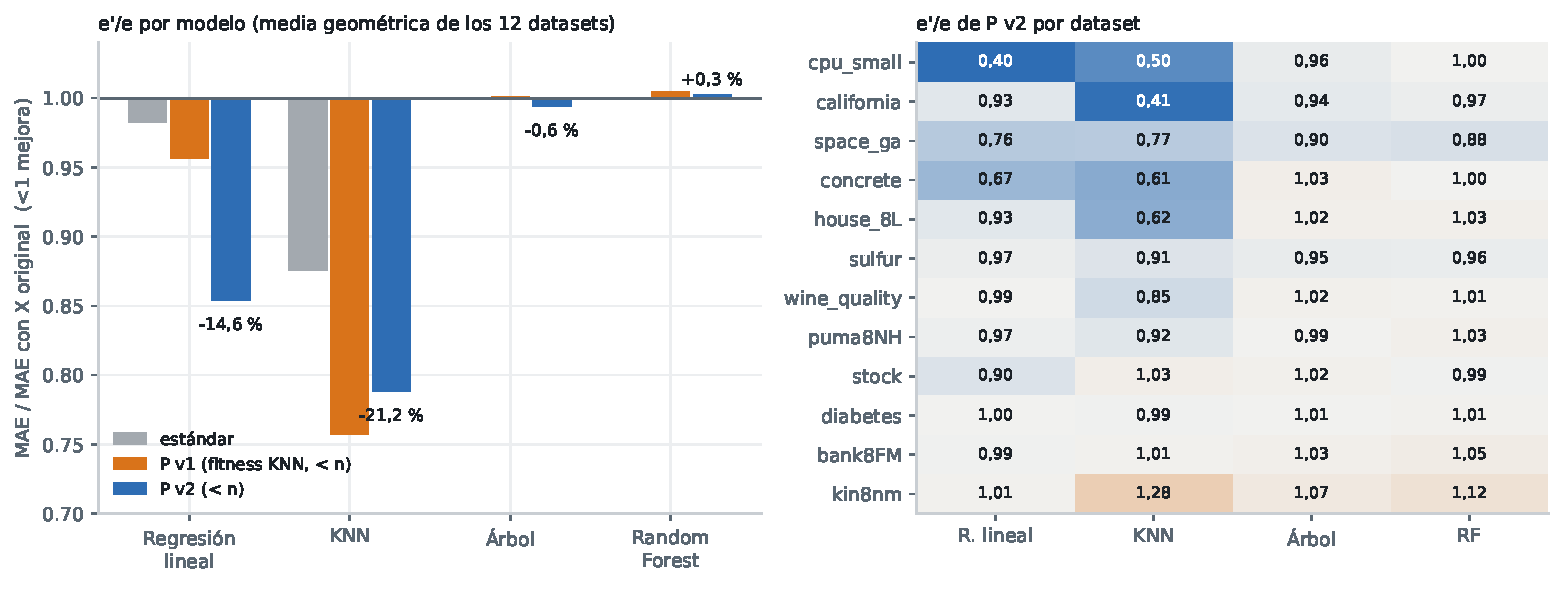
\includegraphics[width=\textwidth]{principal_v2}
\caption{Izquierda: $e'/e$ por modelo. Derecha: $e'/e$ de $P$ v2 por dataset (azul: mejora; naranja: empeora).}
\label{fig:principal}
\end{figure}

\textbf{Reducción.} $X'$ usa el \dosDimMedia{} de los atributos: \dosOrigMedia{} originales y \dosCompMedia{}
componentes de media, con componentes en el \dosFracConComp{} de las particiones (la v1, con fitness solo de KNN, casi
nunca sintetizaba). En kin8nm, donde todos los atributos importan por igual, cambiar originales por componentes
empeora a los cuatro modelos.

\subsection{Comparativa}
\begin{table}[tb]\centering\setlength{\tabcolsep}{4pt}
\caption{Comparativa en las mismas particiones: $e'/e$ (negrita: mejor; $^*$: $P$ v2 mejor con $p<0{,}05$, Wilcoxon por
dataset con Holm), rango medio de Friedman y dimensión relativa $d/n$.}
\label{tab:comparativa}\scriptsize
\begin{tabular}{@{}lcccccc@{}}\toprule
Transformación & R.\ lin. & KNN & Árbol & RF & Rango & $d/n$\\\midrule
\filasComparativaDos\bottomrule
\end{tabular}
\end{table}
$P$ v2 es segunda en rango medio (\dosRangoP), solo por detrás de $P$ sin reducir ($2n$ atributos), y la mejor de las
transformaciones que no aumentan la dimensión (Tabla~\ref{tab:comparativa}). En RL supera significativamente a todas
salvo a la programación genética. Reducir sustituyendo los ejes (``solo PCA'') empeora a RF un \dosCompPCARF.

\subsection{Búsqueda y coste}
En la ablación de la búsqueda de forma y pesos (común a v1 y v2), los pesos son la pieza principal, la búsqueda gana a
la aleatoria (\ctrlAleat{} en KNN) y a los pesos por información mutua (\ctrlMI), y CMA-ES obtiene el mejor rango de
fitness (\rangoCMA) entre siete optimizadores con el mismo presupuesto. Una búsqueda de v2 tarda \dosSegMediana\,s de
mediana por partición (v1: \segMediana\,s) y se paga una vez por dataset.

\section{Conclusiones}
Aumentar el espacio con componentes, ponderar cada candidato y conservar como mucho $n-1$ cumple la reducción de
dimensionalidad con un criterio aprendido por CMA-ES y, con un fitness de tres modelos, produce una representación más
equilibrada que optimizar solo para KNN: gana mucho en regresión lineal a costa de algo de KNN. Los árboles siguen sin
mejorar en media; lo que más les ayuda es añadir dimensiones. Limitaciones: datasets pequeños, casos negativos (kin8nm,
diabetes) y un coste de unos minutos por búsqueda. La parada con datos apartados no compensa a estos tamaños.

\begin{thebibliography}{10}
\bibitem{hansen2001} Hansen, N., Ostermeier, A.: Completely derandomized self-adaptation in evolution strategies.
Evolutionary Computation \textbf{9}(2), 159--195 (2001)
\bibitem{yeo2000} Yeo, I.K., Johnson, R.A.: A new family of power transformations to improve normality or symmetry.
Biometrika \textbf{87}(4), 954--959 (2000)
\bibitem{wettschereck1997} Wettschereck, D., Aha, D.W., Mohri, T.: A review and empirical evaluation of feature
weighting methods for a class of lazy learning algorithms. Artif. Intell. Rev. \textbf{11}, 273--314 (1997)
\bibitem{raymer2000} Raymer, M.L., Punch, W.F., Goodman, E.D., Kuhn, L.A., Jain, A.K.: Dimensionality reduction using
genetic algorithms. IEEE Trans. Evol. Comput. \textbf{4}(2), 164--171 (2000)
\bibitem{weinberger2009} Weinberger, K.Q., Saul, L.K.: Distance metric learning for large margin nearest neighbor
classification. J. Mach. Learn. Res. \textbf{10}, 207--244 (2009)
\bibitem{rodriguez2006} Rodríguez, J.J., Kuncheva, L.I., Alonso, C.J.: Rotation forest: a new classifier ensemble
method. IEEE Trans. Pattern Anal. Mach. Intell. \textbf{28}(10), 1619--1630 (2006)
\bibitem{demsar2006} Demšar, J.: Statistical comparisons of classifiers over multiple data sets. J. Mach. Learn.
Res. \textbf{7}, 1--30 (2006)
\end{thebibliography}
\end{document}
